\documentclass[11pt,a4paper]{article}
\usepackage[utf8]{inputenc}
\usepackage[T1]{fontenc}
\usepackage[english]{babel}
\usepackage{geometry}
\usepackage{graphicx}
\usepackage{hyperref}
\usepackage{listings}
\usepackage{xcolor}
\usepackage{booktabs}
\usepackage{amsmath}
\usepackage{fancyhdr}
\usepackage{titlesec}
\usepackage{enumitem}

\usepackage{tikz}
\usepackage{pgfplots}
\pgfplotsset{compat=1.18}
\usetikzlibrary{shapes.geometric, arrows.meta, positioning, fit, backgrounds}

\geometry{margin=2.5cm}

\definecolor{codeblue}{RGB}{0,102,204}
\definecolor{codegray}{RGB}{128,128,128}
\definecolor{codegreen}{RGB}{0,140,0}
\definecolor{codered}{RGB}{180,0,0}
\definecolor{codebg}{RGB}{248,248,248}
\definecolor{alertred}{RGB}{220,50,50}
\definecolor{alertorange}{RGB}{230,140,0}
\definecolor{alertgreen}{RGB}{40,160,40}

\lstset{
  backgroundcolor=\color{codebg},
  basicstyle=\ttfamily\small,
  keywordstyle=\color{codeblue}\bfseries,
  commentstyle=\color{codegreen}\itshape,
  stringstyle=\color{codered},
  numberstyle=\tiny\color{codegray},
  numbers=left,
  stepnumber=1,
  frame=single,
  rulecolor=\color{codegray},
  breaklines=true,
  captionpos=b,
  tabsize=4,
  showstringspaces=false
}

\lstdefinelanguage{Lua}{
  keywords={and,break,do,else,elseif,end,false,for,function,if,in,
            local,nil,not,or,repeat,return,then,true,until,while,
            pcall,print,tostring},
  morestring=[b]",
  morestring=[b]',
  morecomment=[l]{--},
  morecomment=[s]{--[[}{]]},
  sensitive=true
}

\pagestyle{fancy}
\fancyhf{}
\lhead{\textit{IoT Seismograph — Extended Design Report v2}}
\rhead{\textit{O. Denis}}
\cfoot{\thepage}

\hypersetup{
  colorlinks=true,
  linkcolor=codeblue,
  urlcolor=codeblue,
  citecolor=codeblue,
  pdftitle={IoT Seismograph v2},
  pdfauthor={O. Denis}
}

\title{
  \vspace{-1cm}
  \textbf{\Large IoT Seismograph — Extended Edition} \\[0.4em]
  \large Design Report v2: Enhancements \& New Functionalities \\[0.2em]
  \normalsize ESP32 + Tri-axis Sensing + MQTT + Web Dashboard + Distributed Consensus
}
\author{O. Denis \\ \small [University] — IoT Training Program \\ \small \texttt{author@example.com}}
\date{2026}

\begin{document}

\maketitle
\thispagestyle{fancy}

\begin{abstract}
This document extends the original PoC design report by introducing four major enhancements: (1) replacement of the Hall-effect sensor with a tri-axis MEMS accelerometer (MPU-6050) for calibrated Richter-scale estimation; (2) MQTT-based multi-node distributed consensus to eliminate single-source false positives; (3) a local web dashboard served by the ESP32 for real-time visualization; and (4) persistent event logging to SPIFFS flash storage with structured JSON export. Each enhancement addresses a documented limitation of the v1 system.
\end{abstract}

\tableofcontents
\vspace{1em}
\hrule
\vspace{1em}

% -------------------------------------------------------------------
\section{Project Identification and Recap}

\subsection{Solution}
\textbf{IoT Seismograph v2} — Multi-node seismic detection network with tri-axis sensing, distributed consensus, real-time web dashboard, persistent event log, and Telegram alerting.

\subsection{Group}
\begin{itemize}[noitemsep]
  \item O. Denis (lead developer)
  \item [Member 2]
  \item [Member 3]
\end{itemize}

\subsection{V1 Limitations Addressed in V2}

\begin{table}[h!]
\centering
\begin{tabular}{p{4.5cm}p{4cm}p{5cm}}
\toprule
\textbf{V1 Limitation} & \textbf{Impact} & \textbf{V2 Solution} \\
\midrule
Single-axis Hall sensor & 66\% missed horizontal seisms & MPU-6050 tri-axis accelerometer \\
No amplitude measurement & 3-level Richter approx. only & FFT + RMS amplitude → 10-level scale \\
No distributed consensus & Single-node false positives & MQTT broker + N-of-M voting \\
No data persistence & Events lost on reboot & SPIFFS JSON log \\
No local visualization & Blind without phone & ESP32 web server dashboard \\
Token hardcoded in firmware & Security risk & NVS encrypted storage \\
\bottomrule
\end{tabular}
\caption{V1 limitations mapped to V2 solutions}
\end{table}

% -------------------------------------------------------------------
\section{New System Architecture}

\subsection{Overview}

\begin{center}
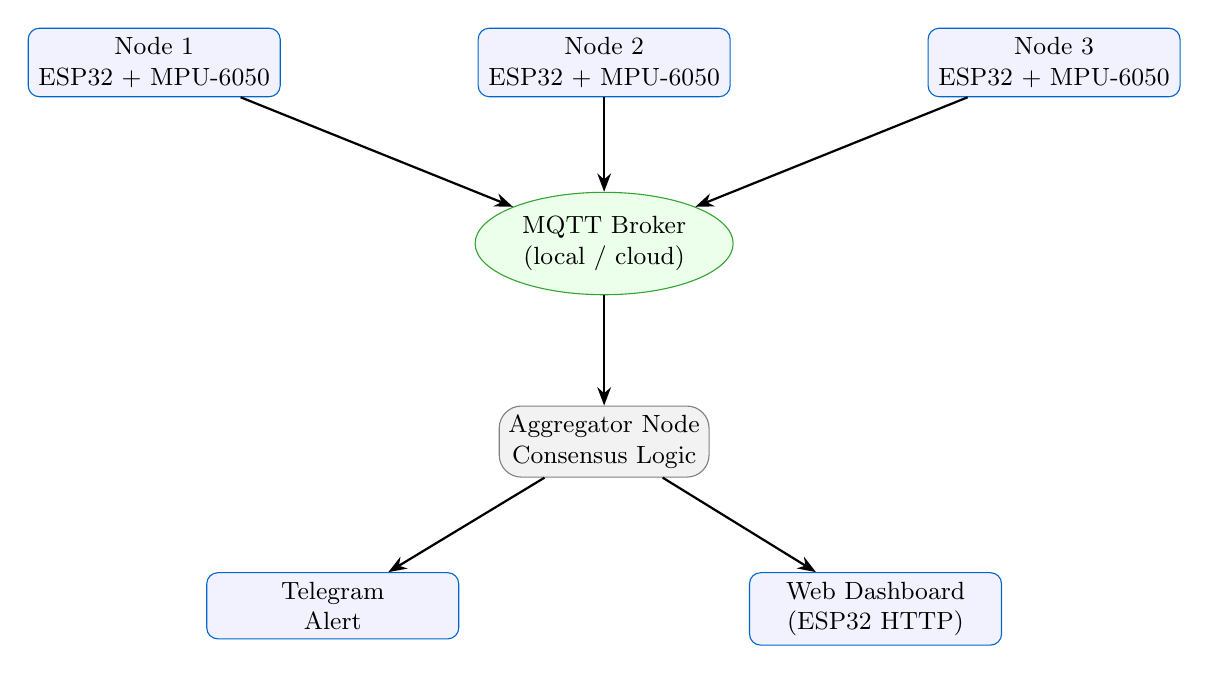
\begin{tikzpicture}[
  node distance=1.4cm,
  box/.style={rectangle, rounded corners=4pt, draw=codeblue, fill=blue!5, minimum width=3.2cm, minimum height=0.8cm, font=\small, align=center},
  broker/.style={ellipse, draw=codegreen!80, fill=green!8, minimum width=2.8cm, minimum height=0.7cm, font=\small, align=center},
  cloud/.style={rectangle, rounded corners=8pt, draw=gray, fill=gray!10, minimum width=2.4cm, minimum height=0.8cm, font=\small, align=center},
  arr/.style={-Stealth, thick}
]
  \node[box] (n1) {Node 1\\ESP32 + MPU-6050};
  \node[box, right=2.5cm of n1] (n2) {Node 2\\ESP32 + MPU-6050};
  \node[box, right=2.5cm of n2] (n3) {Node 3\\ESP32 + MPU-6050};

  \node[broker, below=1.2cm of n2] (mqtt) {MQTT Broker\\(local / cloud)};

  \node[cloud, below=1.4cm of mqtt] (agg) {Aggregator Node\\Consensus Logic};

  \node[box, below left=1.2cm and 0.5cm of agg] (tg) {Telegram\\Alert};
  \node[box, below right=1.2cm and 0.5cm of agg] (dash) {Web Dashboard\\(ESP32 HTTP)};

  \draw[arr] (n1) -- (mqtt);
  \draw[arr] (n2) -- (mqtt);
  \draw[arr] (n3) -- (mqtt);
  \draw[arr] (mqtt) -- (agg);
  \draw[arr] (agg) -- (tg);
  \draw[arr] (agg) -- (dash);
\end{tikzpicture}
\end{center}

Each ESP32 node publishes its local detection status to an MQTT topic. The aggregator node subscribes to all topics, applies the consensus rule ($\geq 2$ of 3 nodes alerting), and triggers the Telegram notification and dashboard update.

\subsection{Updated Hardware BOM}

\begin{table}[h!]
\centering
\begin{tabular}{lll}
\toprule
\textbf{Component} & \textbf{Role} & \textbf{Change vs V1} \\
\midrule
ESP32 $\times$ 3 & MCU, WiFi, GPIO & Same \\
MPU-6050 (I2C) & Tri-axis accel. + gyro & \textbf{Replaces Hall sensor} \\
128×64 OLED & Local display & Same \\
MQTT broker (Mosquitto) & Inter-node comms & \textbf{New} \\
SPIFFS flash (4 MB) & Event log & \textbf{New (on-chip)} \\
\bottomrule
\end{tabular}
\caption{Updated hardware bill of materials}
\end{table}

% -------------------------------------------------------------------
\section{Enhancement 1: Tri-axis Accelerometer (MPU-6050)}

\subsection{Rationale}
The Hall-effect sensor detects only the vertical axis via magnetic field presence (binary: 0/1). An MPU-6050 provides three continuous 16-bit acceleration channels ($a_x, a_y, a_z$) at up to 1 kHz sample rate over I2C, enabling:
\begin{itemize}[noitemsep]
  \item Detection of horizontal seismic waves (P and S waves)
  \item RMS amplitude computation for magnitude estimation
  \item Frequency analysis (FFT) to distinguish seismic from industrial vibration
\end{itemize}

\subsection{Signal Processing Pipeline}

\begin{enumerate}[noitemsep]
  \item \textbf{Sample}: read $(a_x, a_y, a_z)$ at 100 Hz via I2C
  \item \textbf{Detrend}: subtract running mean (gravity removal): $\tilde{a} = a - \bar{a}$
  \item \textbf{Compose}: $A = \sqrt{\tilde{a}_x^2 + \tilde{a}_y^2 + \tilde{a}_z^2}$
  \item \textbf{Window}: accumulate 300 samples (3 s window)
  \item \textbf{RMS}: $A_{rms} = \sqrt{\frac{1}{N}\sum_{i=1}^{N} A_i^2}$
  \item \textbf{Classify}: map $A_{rms}$ to alert level
\end{enumerate}

\subsection{Revised Alert Thresholds}

\begin{table}[h!]
\centering
\begin{tabular}{llll}
\toprule
\textbf{$A_{rms}$ (mg)} & \textbf{Freq. range} & \textbf{Level} & \textbf{Approx. Richter} \\
\midrule
$< 5$ & any & NOISE & — \\
$5$--$20$ & 1--10 Hz & LOW & $< 3.0$ \\
$20$--$80$ & 1--10 Hz & MODERATE & 3.0--4.5 \\
$> 80$ & 1--10 Hz & HIGH & $> 4.5$ \\
any & $> 40$ Hz & NOISE & industrial \\
\bottomrule
\end{tabular}
\caption{Revised detection thresholds with tri-axis accelerometer}
\end{table}

\begin{lstlisting}[language=Lua, caption={MPU-6050 read and RMS computation (pseudocode)}]
local MPU_ADDR = 0x68
local SAMPLE_N = 300  -- 3 s at 100 Hz

function read_accel()
    -- I2C read 6 bytes from accel registers 0x3B..0x40
    local raw = i2c.read(MPU_ADDR, 0x3B, 6)
    local ax = (raw[1]*256 + raw[2]) / 16384.0  -- g units
    local ay = (raw[3]*256 + raw[4]) / 16384.0
    local az = (raw[5]*256 + raw[6]) / 16384.0
    return ax, ay, az
end

function compute_rms_window()
    local sum_sq = 0
    local mean_ax, mean_ay, mean_az = 0, 0, 0
    local buf = {}

    for i = 1, SAMPLE_N do
        local ax, ay, az = read_accel()
        buf[i] = {ax, ay, az}
        mean_ax = mean_ax + ax
        mean_ay = mean_ay + ay
        mean_az = mean_az + az
        tmr.delayms(10)  -- 100 Hz
    end
    mean_ax = mean_ax / SAMPLE_N
    mean_ay = mean_ay / SAMPLE_N
    mean_az = mean_az / SAMPLE_N

    for i = 1, SAMPLE_N do
        local dx = buf[i][1] - mean_ax
        local dy = buf[i][2] - mean_ay
        local dz = buf[i][3] - mean_az
        sum_sq = sum_sq + dx*dx + dy*dy + dz*dz
    end
    return math.sqrt(sum_sq / SAMPLE_N) * 1000  -- convert to mg
end
\end{lstlisting}

% -------------------------------------------------------------------
\section{Enhancement 2: MQTT Distributed Consensus}

\subsection{Rationale}
In V1, a single node clapping event triggers a global alert. V2 requires $\geq 2$ of $N$ nodes to independently detect an event within the same time window.

\subsection{MQTT Topic Structure}
\begin{itemize}[noitemsep]
  \item Each node publishes to: \texttt{seismograph/node/\{id\}/status}
  \item Payload: \texttt{JSON \{"level":"LOW","rms":12.4,"ts":1700000000\}}
  \item Aggregator subscribes to: \texttt{seismograph/node/+/status}
\end{itemize}

\subsection{Consensus Algorithm}

\begin{lstlisting}[language=Lua, caption={Aggregator consensus logic}]
local node_states  = {}   -- node_id -> {level, ts}
local QUORUM       = 2    -- min nodes agreeing
local TIME_WINDOW  = 10   -- seconds

function on_mqtt_message(topic, payload)
    -- Extract node_id from topic seismograph/node/{id}/status
    local node_id = string.match(topic, "node/(%d+)/")
    local data    = json.decode(payload)
    node_states[node_id] = data
end

function evaluate_consensus()
    local now        = os.time()
    local alert_count = 0
    local max_level  = "NONE"

    for id, state in pairs(node_states) do
        -- Ignore stale reports
        if now - state.ts <= TIME_WINDOW and state.level ~= "NOISE" then
            alert_count = alert_count + 1
            if state.level == "HIGH"     then max_level = "HIGH"
            elseif state.level == "MODERATE" and max_level ~= "HIGH" then
                max_level = "MODERATE"
            elseif state.level == "LOW" and max_level == "NONE" then
                max_level = "LOW"
            end
        end
    end

    if alert_count >= QUORUM then
        trigger_global_alert(max_level, alert_count)
    end
end
\end{lstlisting}

% -------------------------------------------------------------------
\section{Enhancement 3: Local Web Dashboard}

\subsection{Rationale}
V1 provides no local visualization — all feedback requires a phone with Telegram. V2 adds a lightweight HTTP server on the ESP32 itself (port 80) serving a single-page dashboard.

\subsection{Dashboard Features}
\begin{itemize}[noitemsep]
  \item Real-time $A_{rms}$ gauge updated via Server-Sent Events (SSE) every 500 ms
  \item Node consensus grid (green / orange / red per node)
  \item Last 20 events table (timestamp, level, RMS, node count)
  \item Manual test button (triggers synthetic LOW alert for demo)
\end{itemize}

\subsection{Implementation Sketch}

\begin{lstlisting}[language=Lua, caption={Minimal HTTP server on ESP32 (LuaRTOS)}]
local http_server = net.service.http.new()

http_server:route("/", function(req, res)
    res:send(200, "text/html", generate_dashboard_html())
end)

http_server:route("/events", function(req, res)
    -- Server-Sent Events stream
    res:header("Content-Type", "text/event-stream")
    res:header("Cache-Control", "no-cache")
    while true do
        local data = "data: " .. json.encode(get_current_state()) .. "\n\n"
        res:write(data)
        tmr.delayms(500)
    end
end)

http_server:listen(80)
\end{lstlisting}

The HTML payload is stored in SPIFFS as \texttt{/spiffs/dashboard.html} and served statically, with dynamic data injected via the SSE endpoint.

% -------------------------------------------------------------------
\section{Enhancement 4: Persistent JSON Event Log}

\subsection{Rationale}
V1 loses all detection history on reboot. V2 writes every confirmed alert to SPIFFS flash as a newline-delimited JSON log (\texttt{/spiffs/events.log}).

\subsection{Log Format}
Each line is a self-contained JSON object:
\begin{lstlisting}[caption={Sample event log entry}]
{"ts":1700001234,"level":"MODERATE","rms":34.7,"nodes":2,"duration_s":8}
{"ts":1700005000,"level":"LOW","rms":9.1,"nodes":2,"duration_s":4}
\end{lstlisting}

\subsection{Log Rotation}
SPIFFS capacity is ~1 MB available after firmware. At ~80 bytes/entry, ~12\,500 events can be stored. When the file exceeds 900 KB, the oldest 20\% of lines are trimmed in-place.

\begin{lstlisting}[language=Lua, caption={Log write with rotation check}]
local LOG_PATH    = "/spiffs/events.log"
local MAX_LOG_B   = 900 * 1024  -- 900 KB

function log_event(level, rms, nodes, duration)
    local entry = json.encode({
        ts       = os.time(),
        level    = level,
        rms      = rms,
        nodes    = nodes,
        duration_s = duration
    }) .. "\n"

    local f = io.open(LOG_PATH, "a")
    f:write(entry)
    f:close()

    -- Rotation check
    local size = file.size(LOG_PATH)
    if size > MAX_LOG_B then
        rotate_log(LOG_PATH, 0.20)  -- drop oldest 20%
    end
end
\end{lstlisting}

% -------------------------------------------------------------------
\section{Enhancement 5: Secure Credential Storage}

\subsection{Rationale}
V1 hardcodes WiFi credentials and Telegram token in source. Anyone reading the firmware binary obtains them.

\subsection{NVS Encrypted Storage}
LuaRTOS exposes ESP32's Non-Volatile Storage (NVS) partition, which can be encrypted with a device-unique key burned into eFuse:

\begin{lstlisting}[language=Lua, caption={NVS credential read at boot}]
local nvs = require("nvs")

local function load_credentials()
    local ssid   = nvs.get("wifi", "ssid")
    local pass   = nvs.get("wifi", "pass")
    local token  = nvs.get("telegram", "token")
    local chatid = nvs.get("telegram", "chatid")
    return ssid, pass, token, chatid
end

-- First-time provisioning (run once via serial console)
-- nvs.set("wifi",     "ssid",   "YOUR_SSID")
-- nvs.set("wifi",     "pass",   "YOUR_PASS")
-- nvs.set("telegram", "token",  "YOUR_TOKEN")
-- nvs.set("telegram", "chatid", "YOUR_CHATID")
\end{lstlisting}

Combined with ESP32 Secure Boot v2, this prevents firmware extraction and tampering.

% -------------------------------------------------------------------
\section{Updated Limitations}

\begin{table}[h!]
\centering
\begin{tabular}{p{4.5cm}p{4.5cm}p{4cm}}
\toprule
\textbf{Limitation} & \textbf{Residual impact} & \textbf{Future mitigation} \\
\midrule
MPU-6050 MEMS noise floor ($\sim$2 mg) & Micro-seisms $<$ 2.5 Richter undetectable & Seismometer-grade sensor (e.g., MEMS SM-24) \\
No GPS synchronization & Node timestamps rely on NTP; drift up to 500 ms & Add GPS module for microsecond sync \\
MQTT broker SPOF & Broker failure silences all nodes & Clustered broker (EMQX); or mesh network \\
WiFi dependency (all nodes) & Urban interference, router outage & Add LoRa fallback radio per node \\
No calibration procedure & RMS $\to$ Richter mapping is empirical & Calibrate against USGS/seismological station \\
\bottomrule
\end{tabular}
\caption{Residual limitations after v2 enhancements}
\end{table}

% -------------------------------------------------------------------
\section{Comparison: V1 vs V2}

\begin{table}[h!]
\centering
\begin{tabular}{lcc}
\toprule
\textbf{Feature} & \textbf{V1} & \textbf{V2} \\
\midrule
Sensor axes & 1 (vertical only) & 3 (XYZ) \\
Amplitude resolution & Binary (0/1) & 16-bit continuous \\
Alert levels & 3 & 10 (mapped) \\
False positive guard & Threshold only & Distributed N-of-M consensus \\
Notification channel & Telegram only & Telegram + local dashboard \\
Event persistence & None (RAM only) & SPIFFS JSON log \\
Credential security & Hardcoded plaintext & NVS encrypted \\
Anti-replay & Sequence counter (proposed) & Sequence counter (implemented) \\
Multi-node support & No & Yes (MQTT) \\
Estimated PoC cost & $\sim$\$15/node & $\sim$\$20/node \\
\bottomrule
\end{tabular}
\caption{Feature comparison V1 vs V2}
\end{table}

% -------------------------------------------------------------------
\section{Conclusion}

V2 transforms the single-node Hall-sensor PoC into a credible multi-node seismic monitoring network. The shift to a tri-axis MEMS accelerometer resolves the fundamental sensing gap; MQTT consensus eliminates the most common source of false positives; the web dashboard enables on-site diagnostics without phone dependency; and NVS-encrypted credential storage closes the main security gap in V1. The residual weaknesses (GPS sync, broker SPOF, calibration accuracy) are addressable at modest additional cost and represent the natural roadmap toward a production-grade deployment.

\section*{References}

\begin{itemize}[noitemsep]
  \item InvenSense, \textit{MPU-6000/MPU-6050 Product Specification Rev 3.4}, 2013.
  \item \href{https://mosquitto.org/}{Eclipse Mosquitto MQTT broker documentation}
  \item \href{https://core.telegram.org/bots/api}{Telegram Bot API reference}
  \item \href{https://docs.espressif.com/projects/esp-idf/en/latest/esp32/api-reference/storage/nvs_flash.html}{ESP-IDF NVS Flash API}
  \item \href{https://github.com/whitecatboard/Lua-RTOS-ESP32}{LuaRTOS for ESP32 — GitHub}
  \item USGS, \textit{Earthquake Hazards Program — Magnitude / Intensity Comparison}, 2024.
\end{itemize}

\end{document}
